
\chapter{Evaluating Generated Text}
\label{chap:evaluation}


In this chapter, we introduce two approaches for evaluating semantic accuracy of \ac{d2t} generation.

\section{Evaluating Semantic Accuracy}
\label{sec:sem-acc}

\begin{refbox}
    This section is based on the paper \emph{Evaluating Semantic Accuracy of Data-to-Text Generation with Natural Language Inference} \cite{dusekEvaluatingSemanticAccuracy2020}, joint work with Ondřej Dušek, published in the Proceedings of the The 13th International Conference on Natural Language Generation (INLG 2020). The experimental part was done by Ondřej Dušek, the author of this thesis came up with the initial idea and did the paper writing. The paper has received the award for the best short paper at the conference.
\end{refbox}

In this section, we propose a new metric for evaluating the semantic accuracy of D2T generation. Our metric is based on a neural model pretrained for \ac{nli}.
% : the task of determing whether a hypothesis is true, false, or neutral with respect to a premise. 
We use the \ac{nli} model to check textual entailment between the input data and the output text in both directions, allowing us to reveal omissions or hallucinations.
We demonstrate that even without any extra model training and with minimal handcrafting, our approach achieves high accuracy (>90\%) on the E2E dataset, competitive with scripts specifically handcrafted for the domain, and produces useful results (>75\% accuracy, 0.6 Spearman correlation with human scores) on the more challenging WebNLG dataset. Additionally, we show with manual error analysis that some instances marked as errors were in fact assessed \emph{correctly} by our metric. The experimental code for our metric is available on GitHub.\footnote{\url{https://github.com/ufal/nlgi_eval}}

\subsection{Motivation}

In \ac{d2t} generation, it is essential that the generated text is faithful to the input data. In \autoref{sec:evaluation}, we described two ways how the semantic accuracy of the text can be compromised: the text may be missing some data (\emph{omission}) or contain extra information not supported by the data (\emph{hallucination}).

Since state-of-the-art neural \ac{d2t} generation models are prone to both kinds of errors \cite{gehrmannEndtoEndContentPlan2018,ferreiraNeuralDatatotextGeneration2019,dusekEvaluatingStateoftheartEndtoEnd2020}, recognizing these errors is essential for proper system evaluation and further development. However, it is difficult for handcrafted heuristics to cover all edge cases, as minor changes in wording may cause major differences in the meaning of the text. Human evaluation, on the other hand, is expensive and difficult to scale.

We note that if we transform individual data items to short sentences, we can check whether the each sentence is entailed by the generated text. Specifically, if we find that the sentence is not entailed by the generated text, we can mark this as \emph{omission}. Vice versa, if we concatenate all the simple sentences and these do not entail the generated text; we can mark this as \emph{hallucination}. For this approach, we need only two ingredients: (1) a way to convert individual data items to short sentences, and (2) a model that can check a sentence entailment. We formalize our approach in the next section.



\subsection{Method}
\label{sec:sem-acc:method}
We are given a set of \acs{rdf}\glsunset{rdf} triples $x \in X$, where each triple $x = (s, p, o)$ describes the relation $p$ between the entities $s$ and $o$, and the corresponding natural language description $Y$. Our task is to assess whether $Y$ mentions all the triples in $X$. Additionally, we should also check whether the text mentions any extra information.

\paragraph{Data Preprocessing} Throughout \autoref{chap:low-res}, we have used simple templates for transforming individual triple to \emph{facts}, i.e., simple sentences capturing the meaning of the triple.  We use the same method here, considering two cases:
\begin{enumerate}
    \item \emph{Default:} We use a specific template for each predicate, using templates which are either handcrafted or extracted from the NLG systems' training data.
    \item \emph{Backoff:} We use only a single, universal ``backoff'' template for all the facts, in the form: \emph{The \textless{}predicate\textgreater{} of \textless{}subject\textgreater{} is \textless{}object\textgreater{}}.
\end{enumerate}

\paragraph{Natural Language Inference} \ac{nli} is a sequence classification task which takes two inputs---a \textit{hypothesis} and a \textit{premise}---and produces one of the possible outputs: the hypothesis is \textit{entailed} by (follows from) the premise, \textit{contradicts} the premise, or their relation is \textit{neutral}. Recently, neural models for \ac{nli} \cite{zhang2019semantics,liu-etal-2019-multi,liuRoBERTaRobustlyOptimized2019} reached near-human levels of performance and \ac{nli} was used for evaluating the output of abstractive summarization systems \cite{maynezFaithfulnessFactualityAbstractive2020}.

% Unlike previous works \cite{nie-etal-2019-simple,tian2019sticking,kedzie-mckeown-2019-good}, we use a pretrained neural model finetuned for \ac{nli} which we do not further train on any domain-specific data.

\begin{figure*}[t]
    \centering
    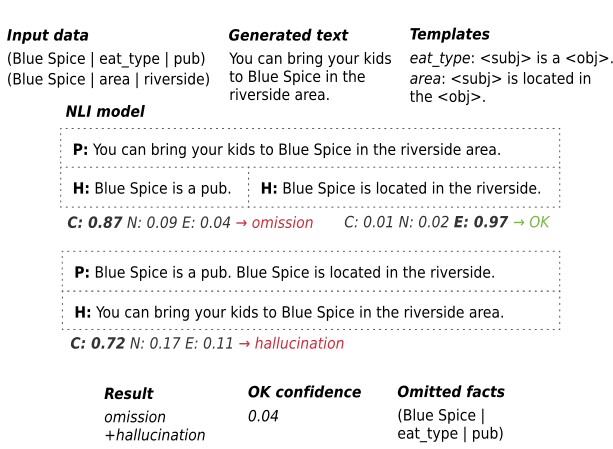
\includegraphics[width=\textwidth]{img/2020_nli_inlg}
    \caption{An example of evaluating the output from a D2T system with our metric. The generated text is used as a \textit{premise} (\textit{P}) to check for omissions and as a \textit{hypothesis} (\textit{H}) to check for hallucinations. The \ac{nli} model generates probabilities for \textit{contradiction} (\textit{C}), \textit{neutral} (\textit{N}) and \textit{entailment} (\textit{E}).}
    \label{fig:sem-acc:ex}
\end{figure*}

\paragraph{Checking Semantic Accuracy with NLI} Consider the two input facts from \autoref{fig:sem-acc:ex}: $F= $\{\emph{``Blue spice is a pub''}, \emph{``Blue Spice is located in the riverside''}\} and the generated text: $Y= $\emph{``You can bring your kids to Blue Spice in the riverside area.''} We propose using a model pretrained for \ac{nli} for checking if the semantic information implied by $F$ and $Y$ is equal.
In this case, the model should detect that the first fact is not entailed by the text (there is no mention of Blue Spice being a pub), but the text is also not entailed by the facts (the information about kids is hallucinated).

We achieve this by using the \ac{nli} model to check for entailment in two directions:
\begin{enumerate}
    \item To check for \textrm{omissions}, we use the whole generated text as a premise and sequentially feed each fact as a hypothesis to the \ac{nli} model. Any failed \ac{nli} check is considered an omission. While we could use all concatenated facts in a single \ac{nli} check, our approach gives us further information about which facts are omitted.
    \item To check for \textrm{hallucinations}, we use a concatenation of all facts as a premise and feed the generated text as a hypothesis to the \ac{nli} model. If this \ac{nli} check fails, the text is considered to contain hallucination. This step cannot be split into simpler \ac{nli} checks.
\end{enumerate}

The final output of our metric is either 4-way (denoted as \textsc{Fine}) or 2-way (denoted as \textsc{Rough}):
\begin{itemize}
    \item \textsc{Fine}: We output the probabilities of 4 categories: \emph{OK} (i.e., all \ac{nli} checks passed), \emph{omission}, \emph{hallucination}, or \emph{omission+hallucination} (based on the failed checks). The 4-way output is more useful for system evaluation, since we can distinguish whether the system tends to hallucinate or omit information.
    \item  \textsc{Rough}: The three incorrect results are collapsed into \emph{not\_OK}. The 2-way output corresponds more to a usage inside an \ac{d2t} generation system for output reranking or filtering: any output that is \emph{not\_OK} should be penalized or filtered out.
\end{itemize}

Additionally, we compute a \textit{confidence score} of the model as the minimum of all the entailment probabilities.


\subsection{Experiments}
\label{sec:sem-acc:experiments}
For our \ac{nli} model, we use the \texttt{roberta-large-mnli}\footnote{\scalebox{0.95}[1.0]{\url{https://huggingface.co/roberta-large-mnli}}} checkpoint of the pretrained RoBERTa model \cite{liuRoBERTaRobustlyOptimized2019}, which was finetuned on the Multi\ac{nli} dataset \cite{williams2018mnli}. We use the model \textit{as is}, without any further training on our side.
Given a premise text and a hypothesis text, the \ac{nli} model produces a probability distribution over three results: \textit{contradiction}, \textit{neutral},
and \textit{entailment} (see \autoref{sec:sem-acc:method}). We consider a \ac{nli} check as passed if the probability for \textit{entailment} is the highest of the three.


We experiment with the WebNLG and E2E datasets (see \autoref{sec:datasets} for details). Since both datasets were used in shared tasks, we can compare the outputs of our system with the respective measures of semantic accuracy:
\begin{itemize}
    \item For WebNLG, we compare our metric with crowdsourced human ratings of semantic adequacy \cite{shimorinaWebNLGChallengeHuman2019}. In particular, we use the question about semantic adequacy: \textit{``Does the text correctly represent the meaning in the data?''}, where the human annotators used a three-point Likert scale (1 = Incorrect, 2 = Medium, 3 = Correct). The answers are averaged over multiple annotators. In our experiments, we consider a sentence correct if it achieved human rating 2.5 or higher.\footnote{We also tried a threshold of 2.0, with slightly worse results.}
    \item For E2E, we compare our metric to the results of the handcrafted automatic script which was used in the E2E challenge \cite{dusekEvaluatingStateoftheartEndtoEnd2020},\footnote{While the E2E challenge did include crowdsourced evaluation of semantic accuracy, the results were unreliable, overestimating the number of errors \cite{dusekEvaluatingStateoftheartEndtoEnd2020}.} We further use small sets of system outputs and human-written texts with expert annotation \citep[provided by][]{dusekSemanticNoiseMatters2019} to evaluate our approach against gold-standard annotation and to compare to existing semantic accuracy classifiers for E2E data.
\end{itemize}


We evaluate the \emph{Default} and \emph{Backoff} approaches to acquiring templates as described in \autoref{sec:sem-acc:method}. The \emph{Default} setup works with one custom template per predicate type. For WebNLG, we obtained templates by delexicalizing human references for single-triple examples from WebNLG training data.\footnote{For each predicate, we choose randomly if more templates are found and use the backoff if no templates are found.} For E2E, we handcrafted 8 templates.
The templates are filled with values from individual input triples and concatenated for multi-triple inputs as described in Section~\ref{sec:eval-process}.

% There's also limited human-annotated system outputs (400) and human-written scripts (200),
% where we can compare to the automatic script.

% =============================================================================
\section{Results Analysis}
\label{sec:results}
% -----------------------------------------------------------------------------


\begin{table}[t]
    \centering \small
    \begin{tabular}{l ccccc>{\hspace{3mm}}ccccc} \toprule
                & \multicolumn{5}{c}{\bfseries WebNLG} & \multicolumn{5}{c}{\bfseries E2E}                                                                                                                  \\
                & \textbf{A}                           & \textbf{R}                        & \textbf{P} & \textbf{F1} & $\mathbf{\rho}$ & \textbf{Af} & \textbf{Ar} & \textbf{R} & \textbf{P} & \textbf{F1} \\\midrule
        Default & 0.775                                & 0.772                             & 0.796      & 0.784       & 0.628           & 0.911       & 0.933       & 0.895      & 0.910      & 0.903       \\
        Backoff & 0.768                                & 0.760                             & 0.793      & 0.776       & 0.637           & 0.846       & 0.874       & 0.913      & 0.768      & 0.834       \\ \bottomrule
    \end{tabular}
    \caption{WebNLG and E2E results, compared to crowdsourced human ratings and the automatic evaluation script, respectively (A = accuracy, Af = \textsc{Fine} accuracy, Ar = \textsc{Rough} accuracy, R = recall, P = precision, F1 = F-measure, $\rho$ = Spearman correlation of confidence scores with human scores).}
    \label{tab:sem-acc:res}
\end{table}




\begin{table*}[t]
    \centering\footnotesize
    \begin{tabular}{@{}l c c ccc >{\hspace{3mm}} c c ccc@{}}\toprule
                          & \multicolumn{5}{c}{\bfseries Human-written (E2E training set)} & \multicolumn{5}{c}{\bfseries System outputs (TGen)}                                                                     \\
                          & \bf Af                                                         & \bf Ar                                              & \bf R & \bf P & \bf F1 & \bf Af & \bf Ar & \bf R & \bf P & \bf F1 \\\midrule
        Slug2Slug aligner & 0.685                                                          & 0.765                                               & 0.550 & 0.800 & 0.652  & 0.995  & 1.000  & 1.000 & 1.000 & 1.000  \\
        E2E script        & 0.820                                                          & 0.885                                               & 1.000 & 0.777 & 0.874  & 0.995  & 0.995  & 1.000 & 0.950 & 0.974  \\
        TGen reranker     & 0.110                                                          & 0.435                                               & 0.975 & 0.413 & 0.579  & 0.220  & 0.278  & 1.000 & 0.116 & 0.208  \\
        \midrule
        Default           & 0.600                                                          & 0.700                                               & 0.625 & 0.625 & 0.625  & 0.978  & 0.978  & 0.947 & 0.837 & 0.888  \\ % 005
        Backoff           & 0.530                                                          & 0.640                                               & 0.675 & 0.540 & 0.600  & 0.833  & 0.833  & 0.974 & 0.359 & 0.525  \\\bottomrule % 006
    \end{tabular}
    \caption{Semantic classifiers evaluated on expert human annotation on E2E data (see \autoref{tab:sem-acc:res} for metrics legend).}
    \label{tab:sem-acc:e2e-slot-comparison}
\end{table*}



% Random baseline would be 0.5 or 0.25 for fine
We evaluate our metric in terms of accuracy, precision, recall, and F1-measure (where \emph{not\_OK} samples are treated as positive since we focus on detecting errors).
We additionally perform a manual error analysis on a random sample of 100 error examples for each dataset, i.e.\ examples where our metric gave a different assessment from the ground truth (provided by crowdsourced annotation for WebNLG and by a handcrafted classification script for E2E as described in Section~\ref{sec:experiments}). % \ZK{zase bych dal poznámku klidně do textu, ať čtenář nemusí tolik skákat}
In general, the results are high above the random baseline (0.5 for the \textsc{Rough} metric and 0.25 for the \textsc{Fine} metric) but differ between the datasets, which we discuss below. %in the following subsections.



% The results for the E2E dataset are better, probably due to the lower lexical variability of the dataset.
% \OD{a možná kvůli tomu, že human eval pro webnlg je trochu zašuměný, ale nevim, jestli se to sem hodí}


% recall is probably more important than precision (not that there are differences)

\subsection{WebNLG Analysis}
\label{sec:webnlg_results}
The overall scores for the WebNLG dataset are summarized in Table \ref{tab:webnlg}. %Here, we compare the \textsc{Rough} metric against the (thresholded) human rating.
To further check whether the size of the input affects performance, we computed Spearman correlation of the number of input triples with metric errors. The resulting very low value of -0.05 ($p=$\,0.02, \emph{Default} setting) shows that the metric holds its performance even for more complex WebNLG examples. %\OD{added this, does it work here?} \ZK{chvilku mi trvalo pochopit, co to číslo počítá, ale asi jo}
%\OD{number of predicates doesn't seem to have a huge effect on performance (1: 78.22, 2: 84.00, 3: 73.55, 4: 77.55, 3: 73.95; spearman -0.0503, p=0.0175)}

%
%
% WebNLG much worse, although still better than random
% not much difference with the backoff templates -- 0.77 vs 0.76
% good correlation with human judgements 0.62-0.63
%
% We can see that the setup using only a backoff template leads to almost the same results as the default setup.
%
%\OD{TODO supplementary should have examples}
%\OD{not much difference w.r.t. backoff means templates are bad}
On the other hand, the overall scores show that our metric deviates quite a lot from the human judgments. Our manual error analysis indicates several reasons for that (see Supplementary for examples): (1) The annotation is somewhat noisy and using a threshold is not ideal---many correctly rendered outputs do not reach the 2.5 threshold (while some incorrect ones do). (2) Imprecise templates can confuse the \ac{nli}
%make the metric check for different information 
(e.g., for the predicate \emph{nationality}, our extracted template is \emph{\textless{}subj\textgreater{} was \textless{}obj\textgreater{}}, which works well with values such as \emph{French}, but not with \emph{United States}). This is currently a weak point of our metric, as illustrated by the very small performance difference between the \emph{Default} and \emph{Backoff} setups; however, the issue can be mitigated by a better selection of the templates from training data, e.g.\ using language-model scoring.
(3) The human annotators tend to give lower scores to accurate but ungrammatical or poorly organized texts. Our metric tends to rate these texts as \emph{OK}.
%Third, we note that many examples are dubious, e.g. there are typos in the text or the text interprets the data too loosely. In these cases, the notion of semantic accuracy can differ between the annotators.
Overall, our re-examination shows that almost half of the error examples (42 out of 100) were in fact correctly classified by our metric (i.e.\ their crowdsourced human annotation was incorrect), %\ZK{přidat něco jako "and not by human evaluators", ať je z toho jasný, že se díváme na chyby a tvrdíme, že to vlastně nejsou chyby?}\OD{takhle dobrý?}
so the true performance is most likely higher than the reported numbers. % due to errors in human annotation.

The Spearman correlation of our model's confidence scores with the average human scores is around 0.63 ($p<$1e-10). This is similar to n-gram-based metrics on this data (\citealp{shimorina_human_2018} reports 0.59 for BLEU and 0.73 for METEOR), but unlike these metrics, our approach does not require human-written reference texts.



\subsection{E2E Analysis}
\label{sec:e2e-results}

% E2E -- very good result -- 0.9 rough, 0.92 fine

% below average prices =~ less than £20
% adult only != not family friendly

% noticeable difference w.r.t. backoff templates

The results for the E2E dataset (shown in Table \ref{tab:e2e}) are very good compared to the WebNLG dataset, with over 90\% agreement with the handcrafted script. This can be attributed to lower lexical variability and less noisy texts, as well as to the better quality of the handcrafted templates (the difference between the \emph{Default} and \emph{Backoff} setups is much more pronounced here).
Again, we observe only a very slight drop in performance for more complex E2E inputs (Spearman correlation of metric errors with the number of input triples is -0.08, $p<$1e-10 for the \emph{Default} setting).
%\OD{only slight drop in performance for more complex inputs (around 96\% rough for up to 5 triples, 93\% for 6 triples, 91\% for 7, spearman 0.07638, p=1.3948e-18)}

%The reference texts often ignore \textit{eatType=restaurant}, which is probably deemed as implicit for the domain. We report the results where we ignore this particular slot-value pair and we observe notable improvements.
%\OD{TODO remove this, incl. from tables}
%\OD{TODO bigger diff w.r.t. backoff, i.e. templates are better}
The main issues identified by our error analysis are:
(1) Problems in the interpretation of some values, e.g., \textit{price range=less than \textsterling{}20} is verbalized as ``cheap'' or \textit{family-friendly=no} as ``adult-only''. These cases are classified as \emph{not\_OK} by the \ac{nli} model.
(2) Missing or over-greedy patterns in the slot error script, causing annotation errors.
(3) Edge cases: some expressions cannot be interpreted in a straightforward way, e.g.\ ``high restaurant'' for \emph{pricerange=high} is deemed OK by the \ac{nli} but not by the slot error script.
(4) Expressions in the outputs that do not correspond to input facts, such as ``with full service'', are considered hallucinations by the \ac{nli}, but ignored by the slot error script.
Again, we consider about half of the error examples (45 out of 100) as correctly classified by our metric (see Supplementary for details), and thus our metric's performance is probably higher than the reported values due to erroneous annotation from the handcrafted script.

% - - - - - - - - - - - - - - - - - - - - - - - - - - - - - - - - - - - - - -
\subsection{E2E MR Classifier Comparison}
% - - - - - - - - - - - - - - - - - - - - - - - - - - - - - - - - - - - - - -
\label{sec:e2e-classifiers}
%As described in Section~\ref{sec:experiments}, there are data in the E2E restaurant domain human-annotated for accuracy (part of the training set, some TGen outputs; \citealp{dusek_semantic_2019}). 
We used expert-annotated E2E data samples (%part of the training set and some system outputs, 
cf.~Section~\ref{sec:experiments}) to compare our approach to other accuracy classifiers in the E2E domain:
\begin{itemize}[nosep,leftmargin=10pt]
    \item \textbf{Slug2Slug slot aligner} \citep{juraska_deep_2018} is based on keyword matches. It is carefully tuned but not designed to detect hallucination; it only checks for presence of facts from the input MR.
    \item \textbf{E2E slot error script} (used in Section~\ref{sec:e2e-results}) is based on regular expressions; it is also able to detect irrelevant facts.
    \item \textbf{TGen reranker} is an LSTM-based model trained on the E2E training data to rerank outputs of the TGen system \cite{dusek_sequence--sequence_2016} based on their semantic accuracy.
          % \item TGen's reranking classifier trained on cleaned E2E data (i.e., reclassified by the slot error script)
\end{itemize}

The results for all classifiers (in Table~\ref{tab:e2e-slot-comparison}) are much weaker on human-written data, which exhibit much more variability than system outputs.
%While the TGen reranker may be useful for relative comparisons of system outputs, it 
The TGen reranker is very weak when required to detect all facts properly.
Our approach is slightly less precise than both handcrafted scripts, but the difference is small on system outputs (97.8\% vs. 99.5\% accuracy). If we disregard the value \emph{eatType=restaurant}, which is generally noisy, we get 76.5\% accuracy and 97.6\% recall on the human-written data. Moreover, our approach requires much less handcrafting and is more general.


\section{Token-Level Error Detection}
\label{sec:eval-token}
\subsection{Shared Task}
\label{sec:eval-st}
\subsection{Our Submission}
\label{sec:eval-ours}